% !TEX root = ../main.tex

\section{Introduction}
\begin{frame}
\frametitle{Neuron dynamics}
\setbeamercovered{transparent}
\onslide<1->{How do neurons communicate?}
\begin{itemize}[<+(1)->]
\item Neurons receive neurotransmitters \\
\item Action potential = explosion of electrical activity \\
\item Synapse releases the neurons' neurotransmitter \\ [0.5cm]
\end{itemize}
\onslide<5->{How can we capture this behaviour?}
\begin{itemize}[<+(2)->]
\item Human brain consists of $\sim$ 100 billion neurons \\
\item The \MFR yields the average dynamics of the network 
\end{itemize}
\end{frame}



\section{The Theta Neuron Model}
\begin{frame}
\frametitle{Model Description}
\tabitem Formulation
\begin{align*}
\dot{\theta} = (1-\cos \theta)+(1+\cos \theta) \cdot I \qquad \theta \in \T 
\end{align*}

\tabitem Normal form of SNIC bifurcation
\begin{figure}[H]
\minipage{0.33\linewidth}
\centering
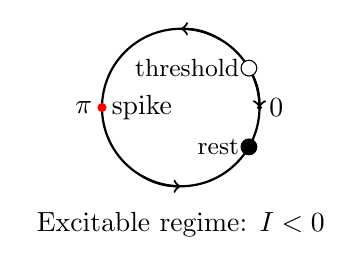
\begin{tikzpicture}
    \draw[thick] (0,0) circle [radius=1];
    \draw (0,-1.2) node[below]{Excitable regime: $I < 0$};
    \draw (-1,0) node[left]{$\pi$};
    \draw[fill=black, black] (1,0) circle [radius=0.025];
    \draw (1,0) node[right]{0};
    \draw[fill=red, red] (-1,0) circle [radius=0.05];
    \draw (-1,0) node[right]{spike};
    
    \draw[black, ->, thick] (0.866, 0.5)to[out=-60,in=90](1,0);
    \draw[fill=white, draw=black] (0.866,0.5) circle [radius=0.1];
    \draw (0.866,0.5) node[left]{\small{threshold}};
    
    \draw[fill=black, draw=black] (0.866,-0.5) circle [radius=0.1];
    \draw (0.866,-0.5) node[left]{\small{rest}};
    
    \draw[black, ->, thick] (0.5,0.866)to[out=150,in=0](0,1);
    \draw[black, ->, thick] (-0.5,-0.866)to[out=-30,in=180](0,-1);
\end{tikzpicture}
\endminipage
\minipage{0.33\linewidth}
\centering
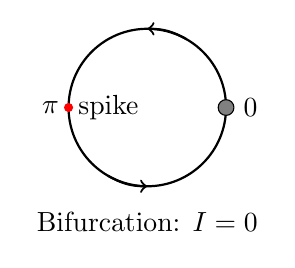
\begin{tikzpicture}
    \draw[thick] (0,0) circle [radius=1];
    \draw (0,-1.2) node[below]{Bifurcation: $I = 0$};
    \draw (1.1,0) node[right]{0};
    \draw[fill=red, red] (-1,0) circle [radius=0.05];
    \draw (-1,0) node[right]{spike};
    \draw (-1,0) node[left]{$\pi$};
    
    \draw[fill=gray, draw=black] (1,0) circle [radius=0.1];
    
    \draw[black, ->, thick] (0.5,0.866)to[out=150,in=0](0,1);
    \draw[black, ->, thick] (-0.5,-0.866)to[out=-30,in=180](0,-1);
\end{tikzpicture}
\endminipage
\minipage{0.33\linewidth}
\centering
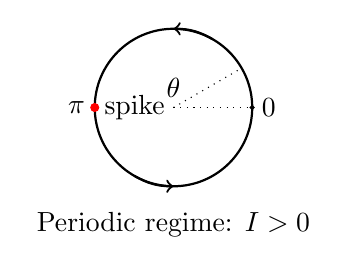
\begin{tikzpicture}
    \draw[thick] (0,0) circle [radius=1];
    \draw (0,-1.2) node[below]{Periodic regime: $I > 0$};
    \draw (-1,0) node[left]{$\pi$};
    \draw (1,0) node[right]{0};
    \draw[fill=black, black] (1,0) circle [radius=0.025];
    \draw[fill=red, red] (-1,0) circle [radius=0.05];
    \draw (-1,0) node[right]{spike};
    
    \draw[black, dotted] (0,0)to(1,0);
    \draw(0,0) node[above]{$\theta$};
    \draw[black, dotted] (0,0)to(0.866,0.5);
    
    \draw[black, ->, thick] (0.5,0.866)to[out=150,in=0](0,1);
    \draw[black, ->, thick] (-0.5,-0.866)to[out=-30,in=180](0,-1);
\end{tikzpicture}
\endminipage
\label{fig:thetaneuronbifurcationtikz}
\end{figure}
\end{frame}

\begin{frame}
\frametitle{Response}
\tabitem Formulate bifurcations in terms of spiking frequency or phase angle
\begin{figure}[H]
\centering
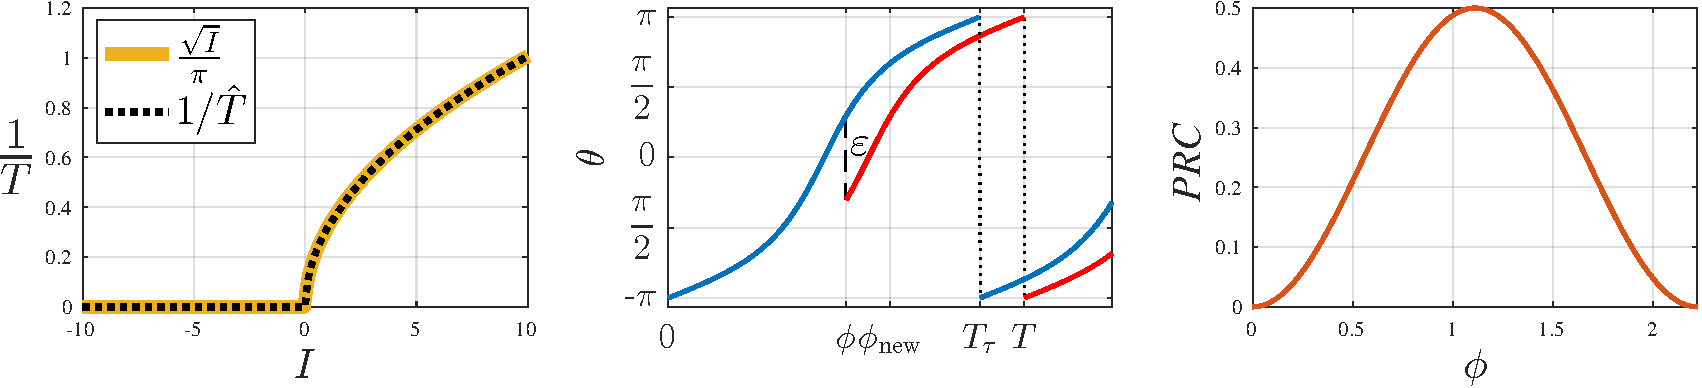
\includegraphics[width = \textwidth]{../Figures/ThetaNeuronfIandPRC.pdf}
\label{fig:ThetaNeuronfIandPRC}
\end{figure}
\end{frame}



\section{Network Topologies}
\begin{frame}
\frametitle{Three basic networks}
\begin{figure}[H]
\centering
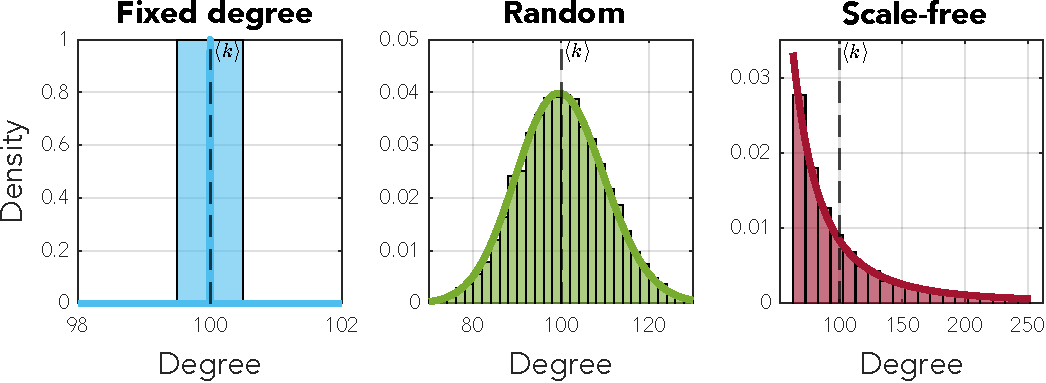
\includegraphics[width = \textwidth]{../Figures/Distributions/1D.pdf}
\label{fig:1Dpdfs}
\end{figure}
\end{frame}

\begin{frame}
\frametitle{Networks of Theta neurons}
\setbeamercovered{transparent}
\onslide<1->{\tabitem For an arbitrary network topology:
\begin{align*}
\dot{\theta}_{i} &=\left(1-\cos \theta_{i}\right)+\left(1+\cos \theta_{i}\right) \cdot \left[\eta_{i} + I_{i}(t)\right] \qquad \theta_i \in \T^N \\
I_{i}(t) &=\frac{\kappa}{\kmean} \sum_{j=1}^{N} A_{i j} \cdot \mathcal{P}_{n}(\theta_{j}) 
\end{align*}
}

\onslide<2->{\tabitem Capture average/mean synchronisation 
\begin{align*}
Z(t) = \frac{1}{N} \sum_{j=1}^N e^{\ic\theta_j}  \qquad Z \in \C 
\end{align*}
}
\end{frame}



\section{Mean Field Reductions}
\begin{frame}
\setbeamercovered{transparent}
\frametitle{Predict synchronisation dynamics} 
The \MFR yields a solution for $Z(t)$\\
\onslide<2->{\tabitem $N$ neurons in the network \\
\tabitem $M_{\k} \ll N$ unique node degrees \\[0.5cm]}

\onslide<3->{Then rewrite $Z(t)$ per degree $z(\k,t)$!\\}
\onslide<4->{\tabitem Only $M_{\k}$ equations \\
\tabitem Weighed by $P(\k)$ \\}
\onslide<5->{
\begin{align*}
\bar{Z}(t) &= \frac{1}{N} \sum_{\k} P(\k) z(\k, t) \qquad \bar{Z} \in \C \label{eq:OttAntonsenMeanField}
\end{align*}
}
\end{frame}

\begin{frame}
\frametitle{Fixed-degree networks}
\begin{figure}[H]
\centering
\begin{subfigure}[b]{0.32\linewidth}
   \centering
  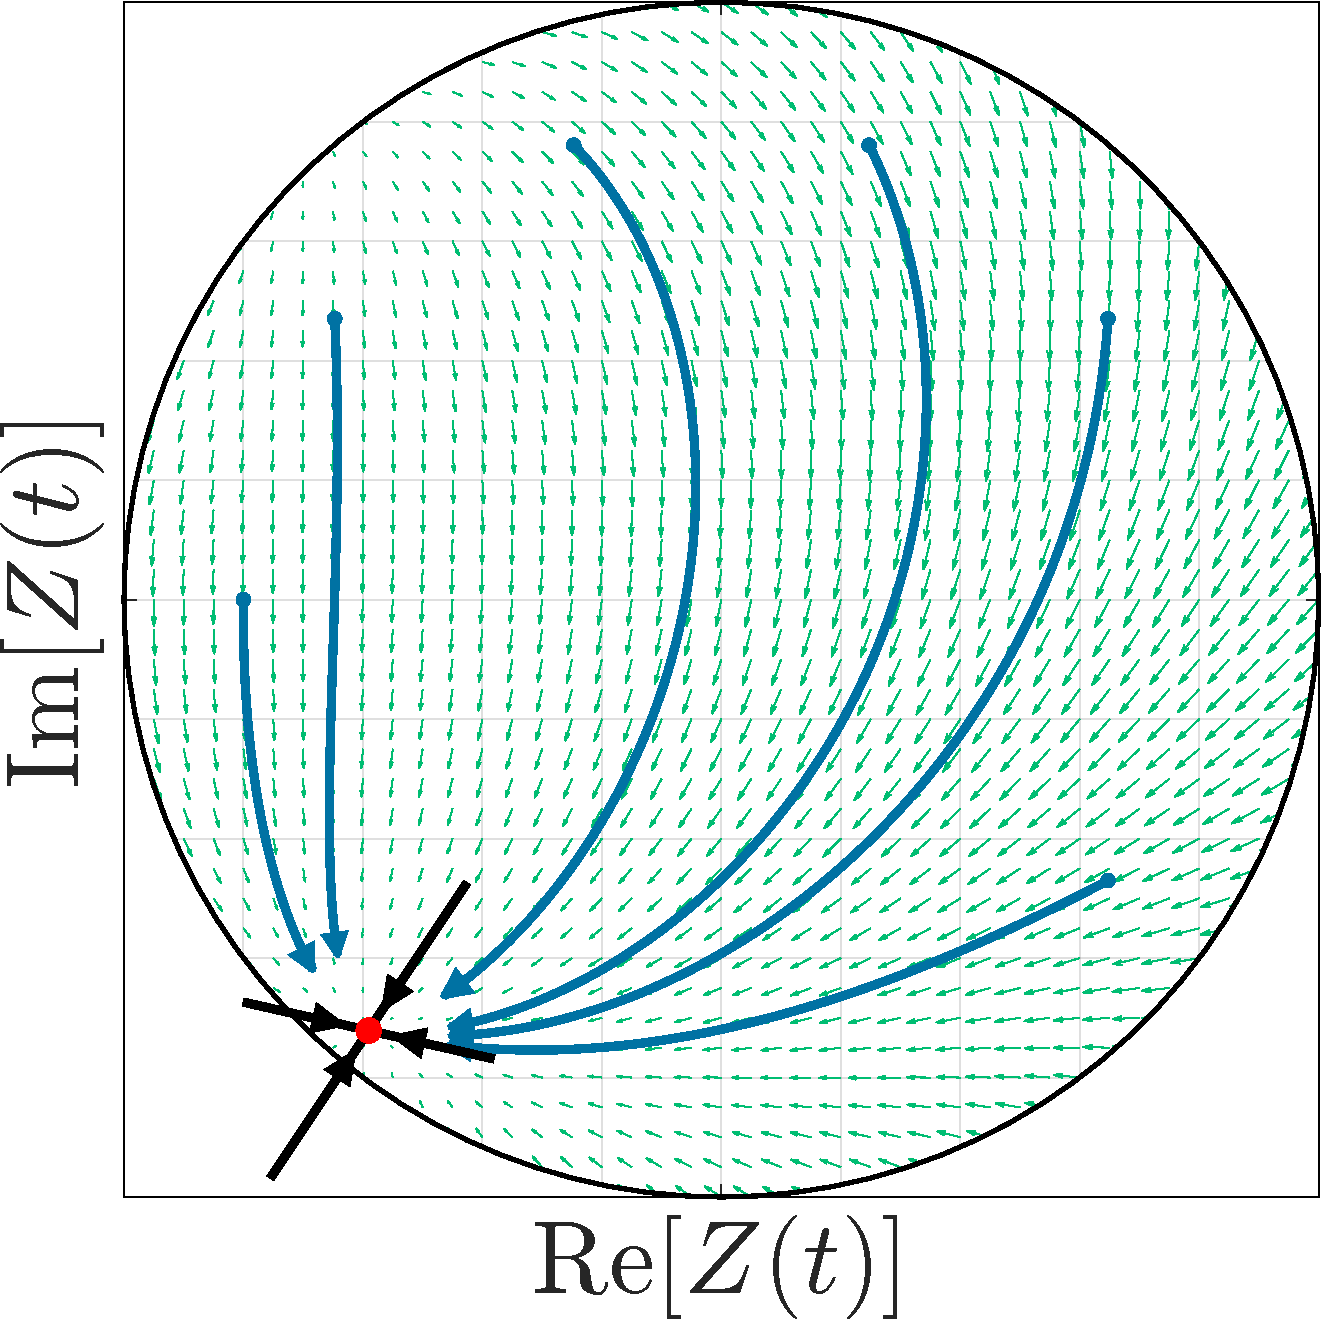
\includegraphics[width=\linewidth]{../Figures/PhaseSpace/MFRPSR.pdf}
   \label{fig:MFRPSR} 
\end{subfigure} \hfill
\begin{subfigure}[b]{0.32\linewidth}
   \centering
  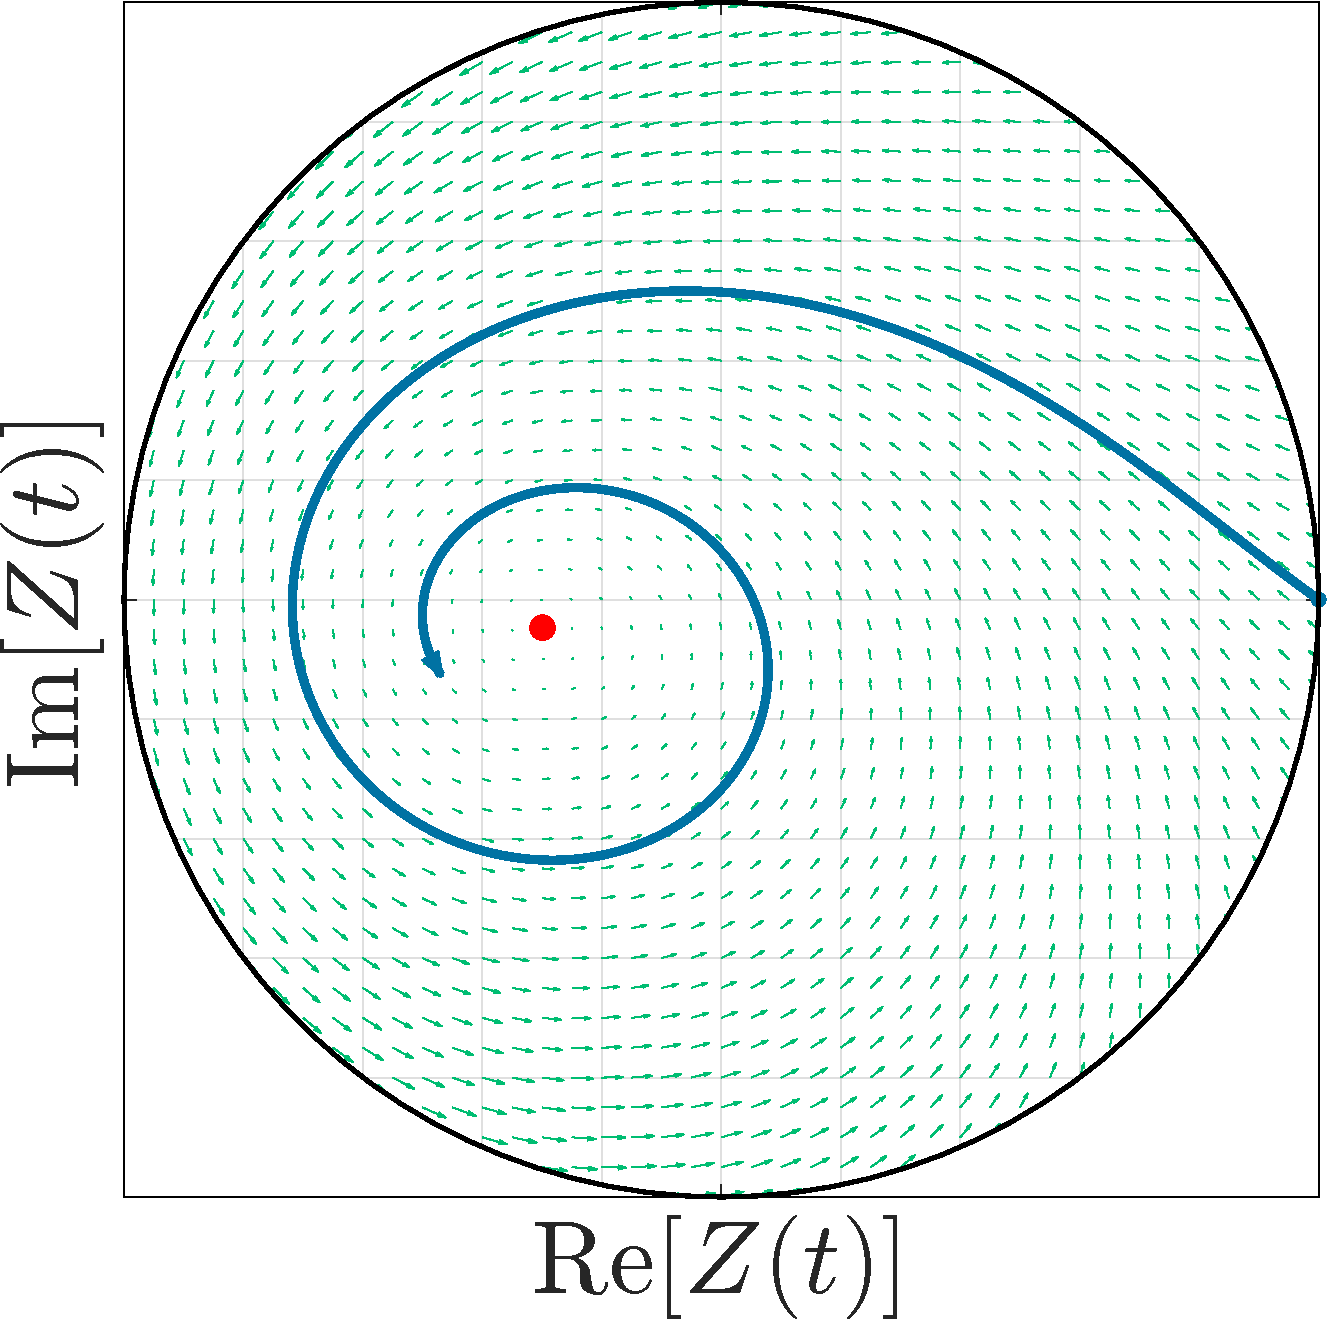
\includegraphics[width=\linewidth]{../Figures/PhaseSpace/MFRPSS.pdf}
   \label{fig:MFRPSS}
\end{subfigure} \hfill
\begin{subfigure}[b]{0.32\linewidth}
   \centering
  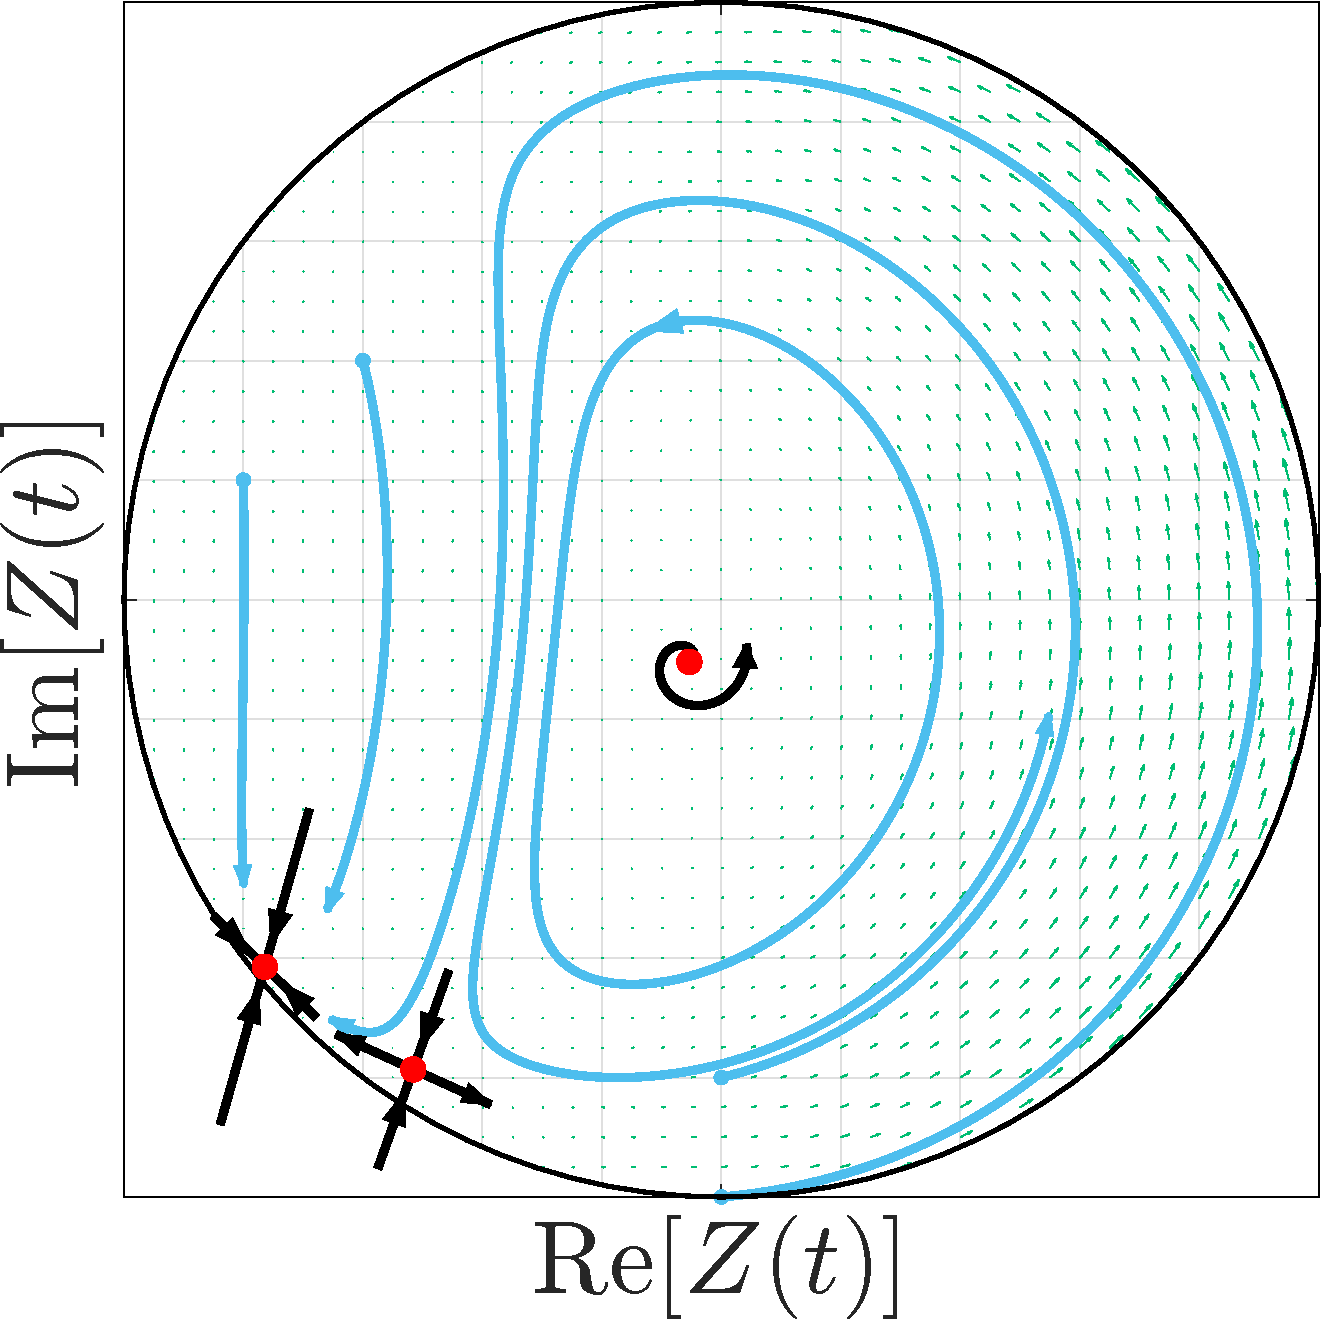
\includegraphics[width=\linewidth]{../Figures/PhaseSpace/MFRCPW.pdf}
   \label{fig:MFRCPW}
\end{subfigure}
   \label{fig:macroscopicstatesfixeddegree}
\end{figure}
\end{frame}

\section{\mywork Mean Field Reductions for undirected graphs} 
\begin{frame}
\setbeamercovered{transparent}
\frametitle{Goals} 
$Z(t)$ can be measured and predicted: are they the same? \\
\begin{itemize}[<+(1)->]
\item Formulate directed networks \\
\item Construct adjacency matrix from degree distribution \\
\item Initial conditions \\
\item Results 
\end{itemize}
\end{frame}

\begin{frame}
\frametitle{Directed networks} 
Use a bivariate degree distribution\\
\tabitem Use identical and independant distributions \\
\tabitem In- and outdegrees are found as a permutation
\end{frame}

\begin{frame}
\frametitle{Directed networks} 
\begin{figure}[ht]
\centering
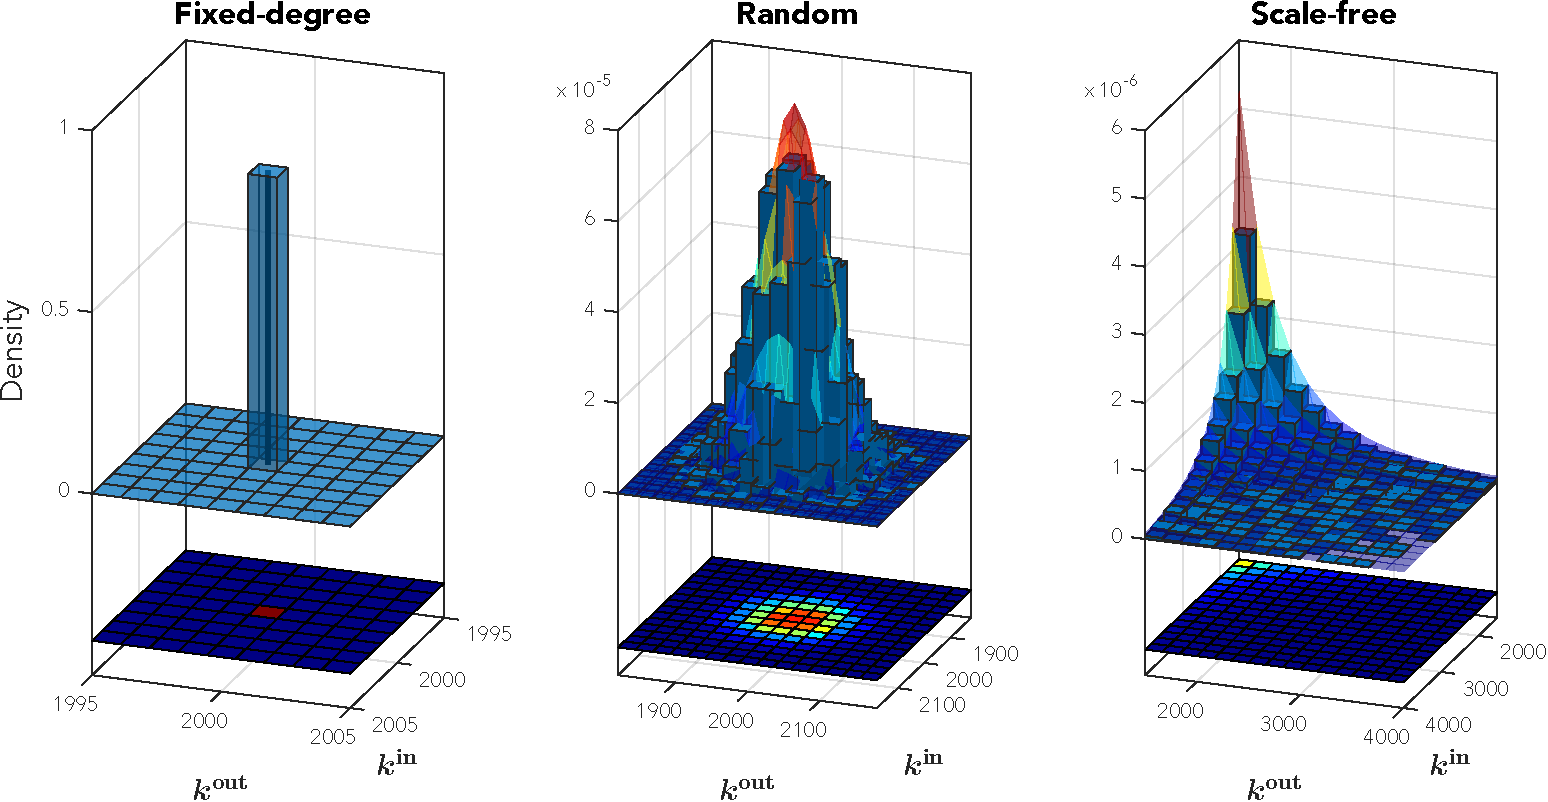
\includegraphics[width = 0.9\textwidth]{../Figures/Distributions/2D.pdf}
\label{fig:2Ddistributions}
\end{figure}
\end{frame}

\begin{frame}
\frametitle{Adjacency matrix} 
Find a probable solution by sampling from the in- and outdegrees
\begin{figure}[H]
\centering
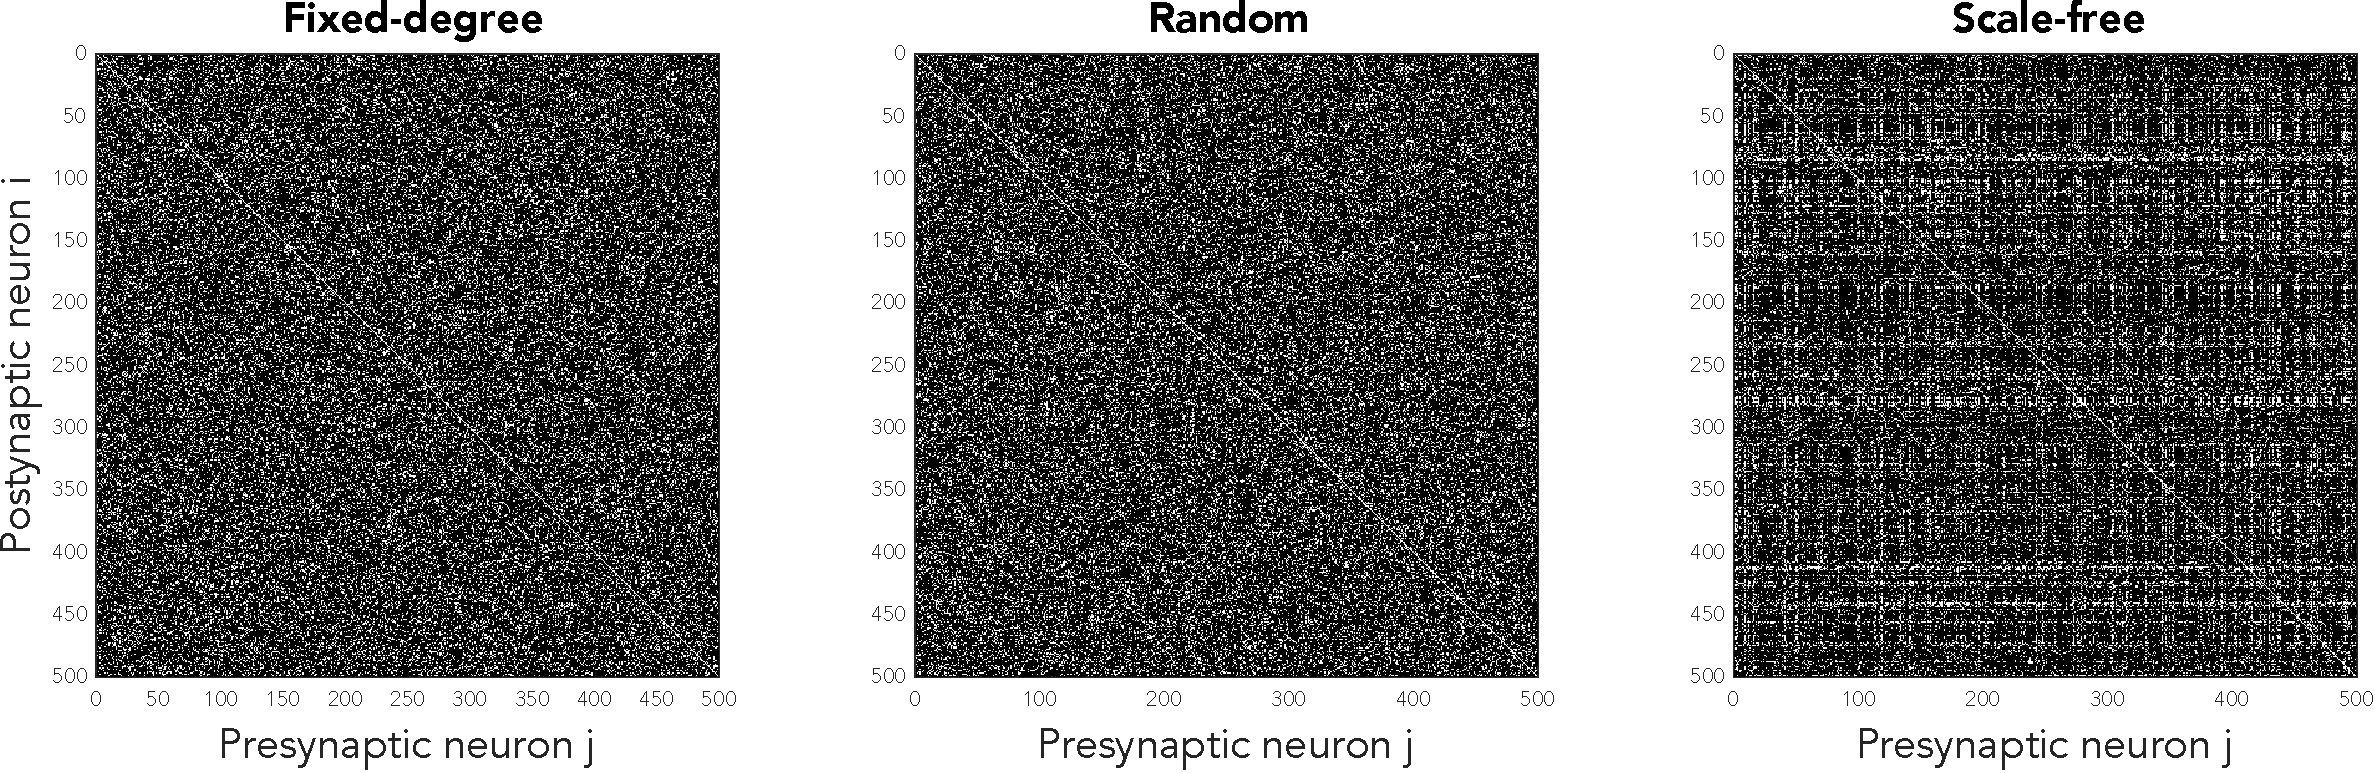
\includegraphics[width = \textwidth]{../Figures/Adjacency_matrices.pdf}
\label{fig:adjacencymatrices}
\end{figure}
\end{frame}

\begin{frame}
\frametitle{Initial conditions} 
\begin{figure}[H]
\centering
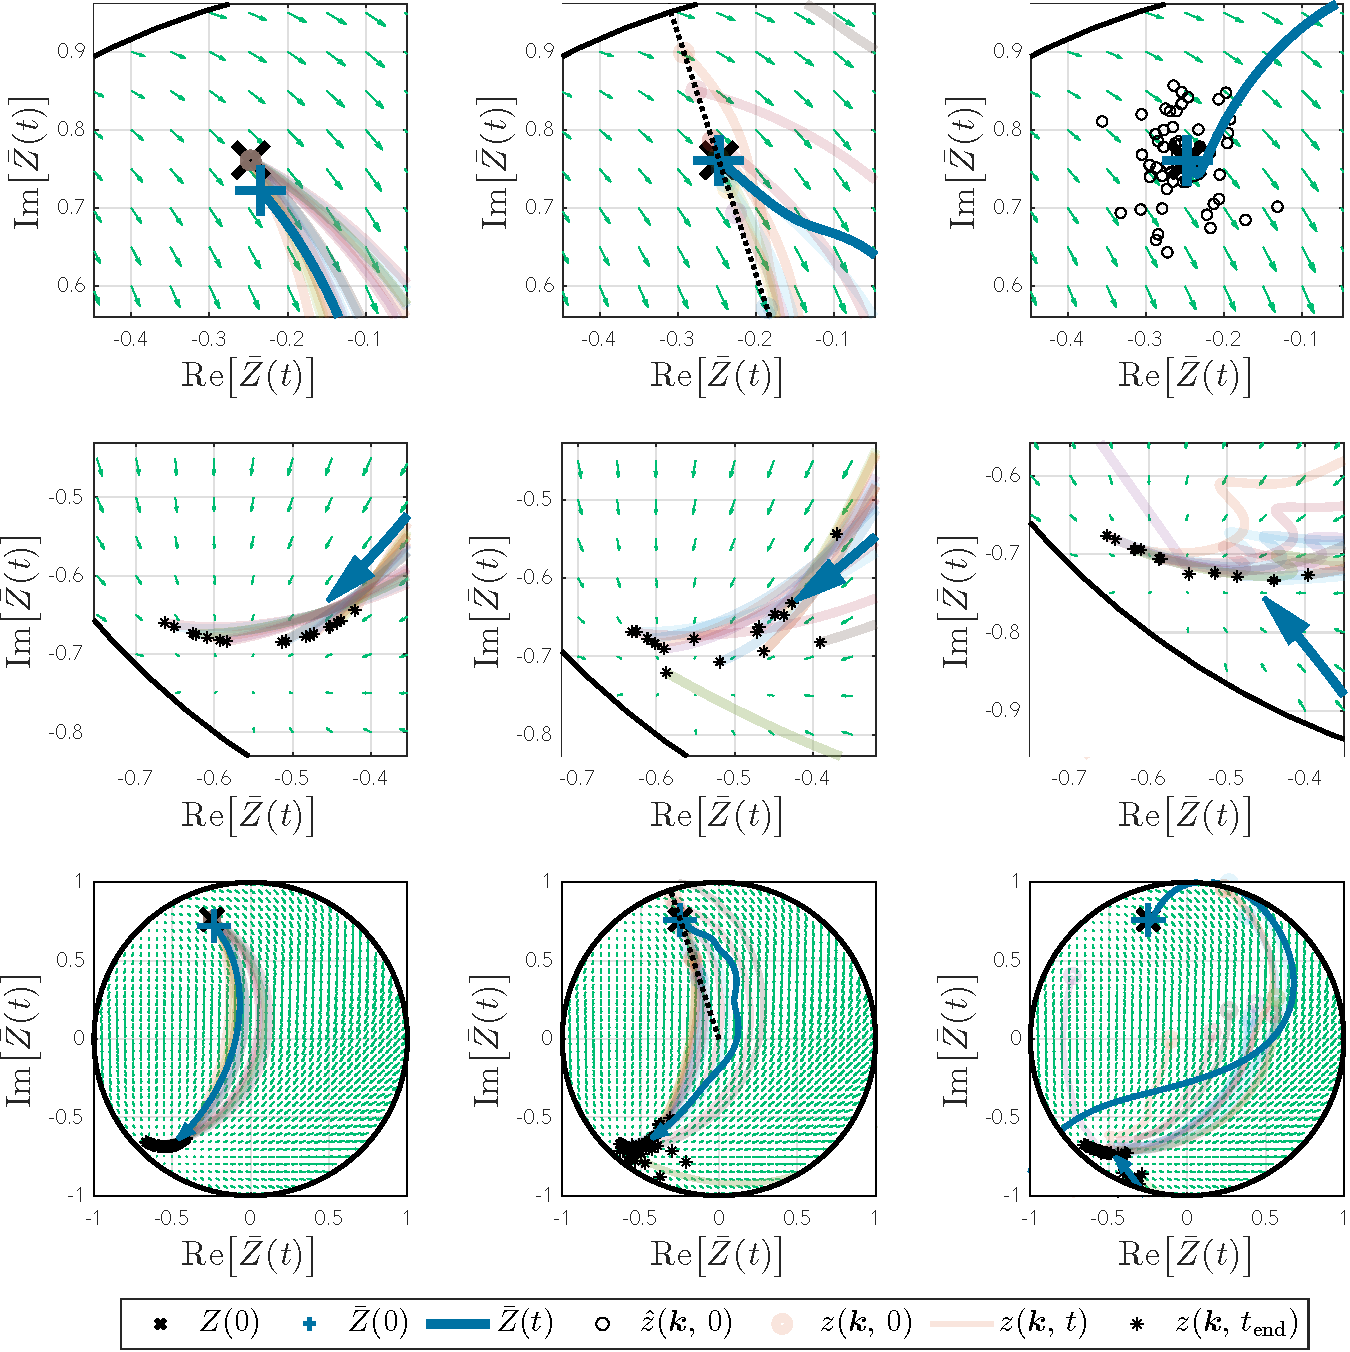
\includegraphics[trim=0cm 8.5cm 0cm 0cm, clip=true, width = 0.75\textwidth]{../Figures/PhaseSpace/Mappings.pdf}
   \label{fig:mappings}
\end{figure}
\end{frame}




\section{Hebbian Learning and Synaptic Plasticity} 
\begin{frame}
\frametitle{Hebbian Learning and Synaptic Plasticity}
\end{frame}


\section{\mywork Emerging Network Topologies} 
\begin{frame}
\frametitle{\mywork Emerging Network Topologies}
\end{frame}


\section{Conclusion and Discussion} 
\begin{frame}
\frametitle{Conclusion and Discussion}
\end{frame}
